\newpage
\chapter{Tests de Diseño}
\label{ch:capitulo5.tex}

\begin{FraseCelebre}
	\begin{Frase}
		Tendrá todo el dinero del mundo, pero hay algo que nunca podrá comprar… un dinosaurio.
	\end{Frase}
	\begin{Fuente}
	Homer J. Simpson
	\end{Fuente}
\end{FraseCelebre}

El objetivo de este capítulo es el de mostrar el resultado de las pruebas de temperaturas realizadas en los diferentes modelos diseñados en el capítulo \ref{ch:capitulo4.tex}. 

\section{Experimental Settings}
\label{makereference5.2}
\paragraph{}

Se ha sometido a estos a un total de tres pruebas, todas ellas con las mismas características para cada modelo, variando en el número de nodos que hay trabajando de forma simultánea en cada caso. De esta manera, según los resultados obtenidos y las características de diseño generadas en el capítulo \ref{ch:capitulo4.tex} determinamos qué modelo es el más idóneo para la elección final.

Además de las pruebas generales, se han realizado una serie de pruebas específicas para cada modelo, el objetivo de estas, ha sido el de determinar la mejor configuración en cuanto a la disposición de los ventiladores dentro del contenedor. En este capítulo, únicamente se muestran las pruebas realizadas a los modelos finales.

Para el desarrollo de cada prueba se ha generado un script que obtiene información de la temperatura del procesador ofrecida directamente por el sistema operativo. El siguiente cuadro muestra el contenido del script:

\begin{lstlisting}[language=c++,frame=single,numbers=none]
	#!/bin/bash
  while test 0 -eq 0 
  do
    sleep $1
    temp=$(/opt/vc/bin/vcgencmd measure_temp | cut -c 6-9)
    time=$(date +"%x" ) #dd/mm/yyyy
    echo "$temp"  
  done
  exit 0
\end{lstlisting}

\section{Prueba 1}
\label{makereference5.3}

\subsection{Escenario}
\paragraph{}

En esta prueba únicamente hay una Raspberry Pi trabajando con cuatro cores, el tiempo total de cada prueba es de tres horas, el periodo de muestreo es de diez segundos y en las gráficas se muestra el tiempo total expresado en segundos. La temperatura ambiente oscila entre los catorce y dieciocho grados. Ninguna de las raspberrys utilizadas dispone de un disipador instalado sobre el procesador.

\subsection{Resultados}

\begin{figure}[H]
	\centering
  	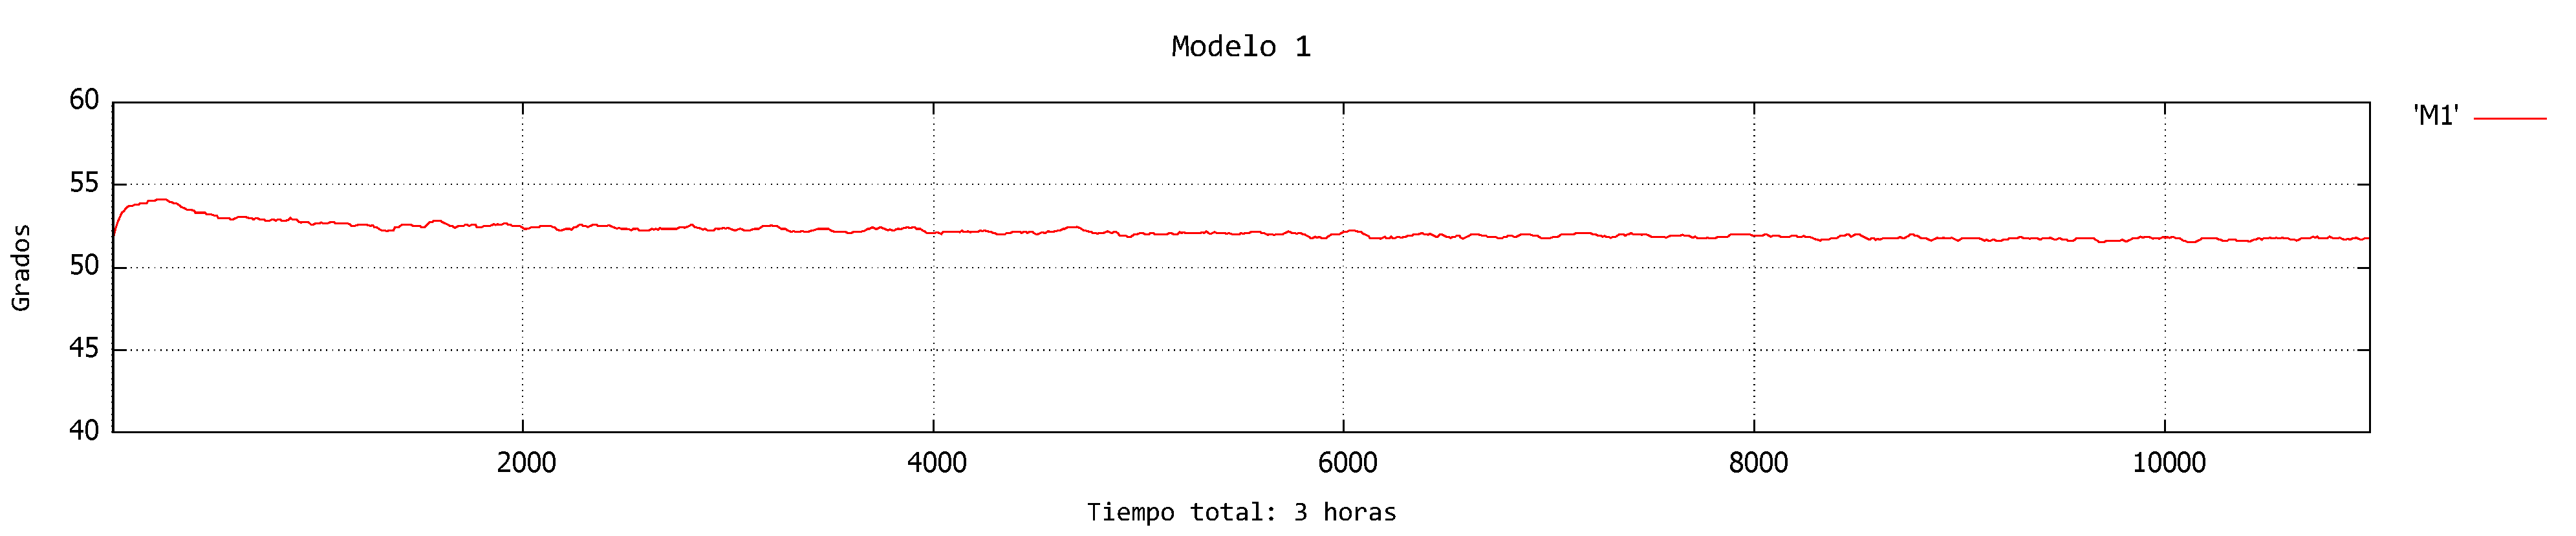
\includegraphics[width=160mm]{Test/Pr1_modelo1.pdf}
   	\caption[Prueba 1, Modelo 1]{Modelo 1}
   \label{figure5.1}
\end{figure}

\begin{figure}[H]
	\centering
  	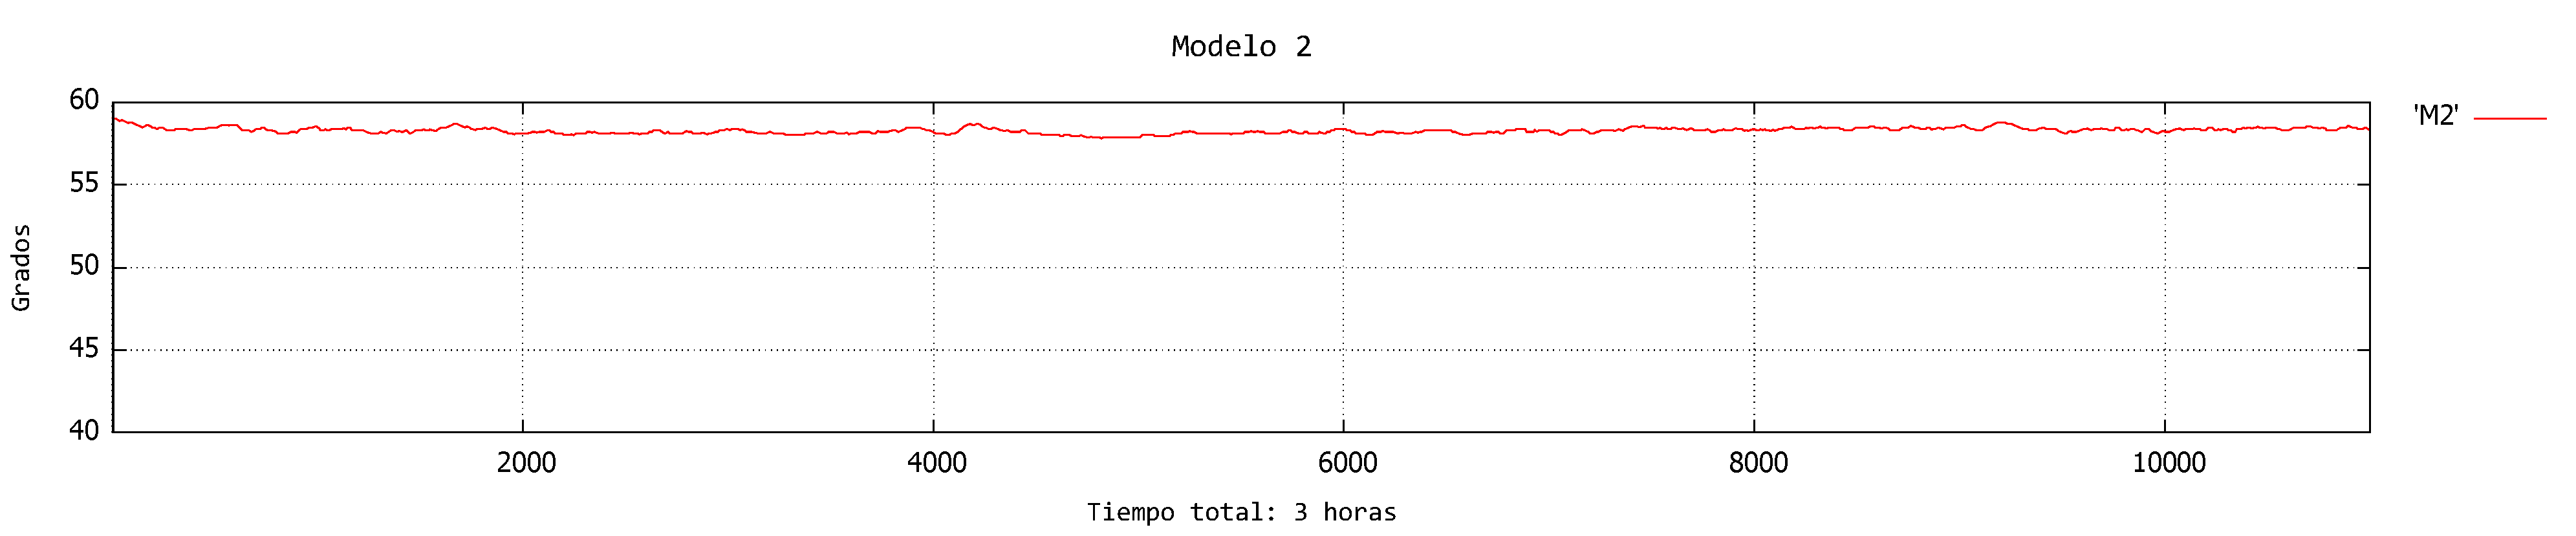
\includegraphics[width=160mm]{Test/Pr1_modelo2.pdf}
   	\caption[Prueba 1, Modelo 2]{Modelo 2}
   \label{figure5.2}
\end{figure}

\begin{figure}[H]
	\centering
  	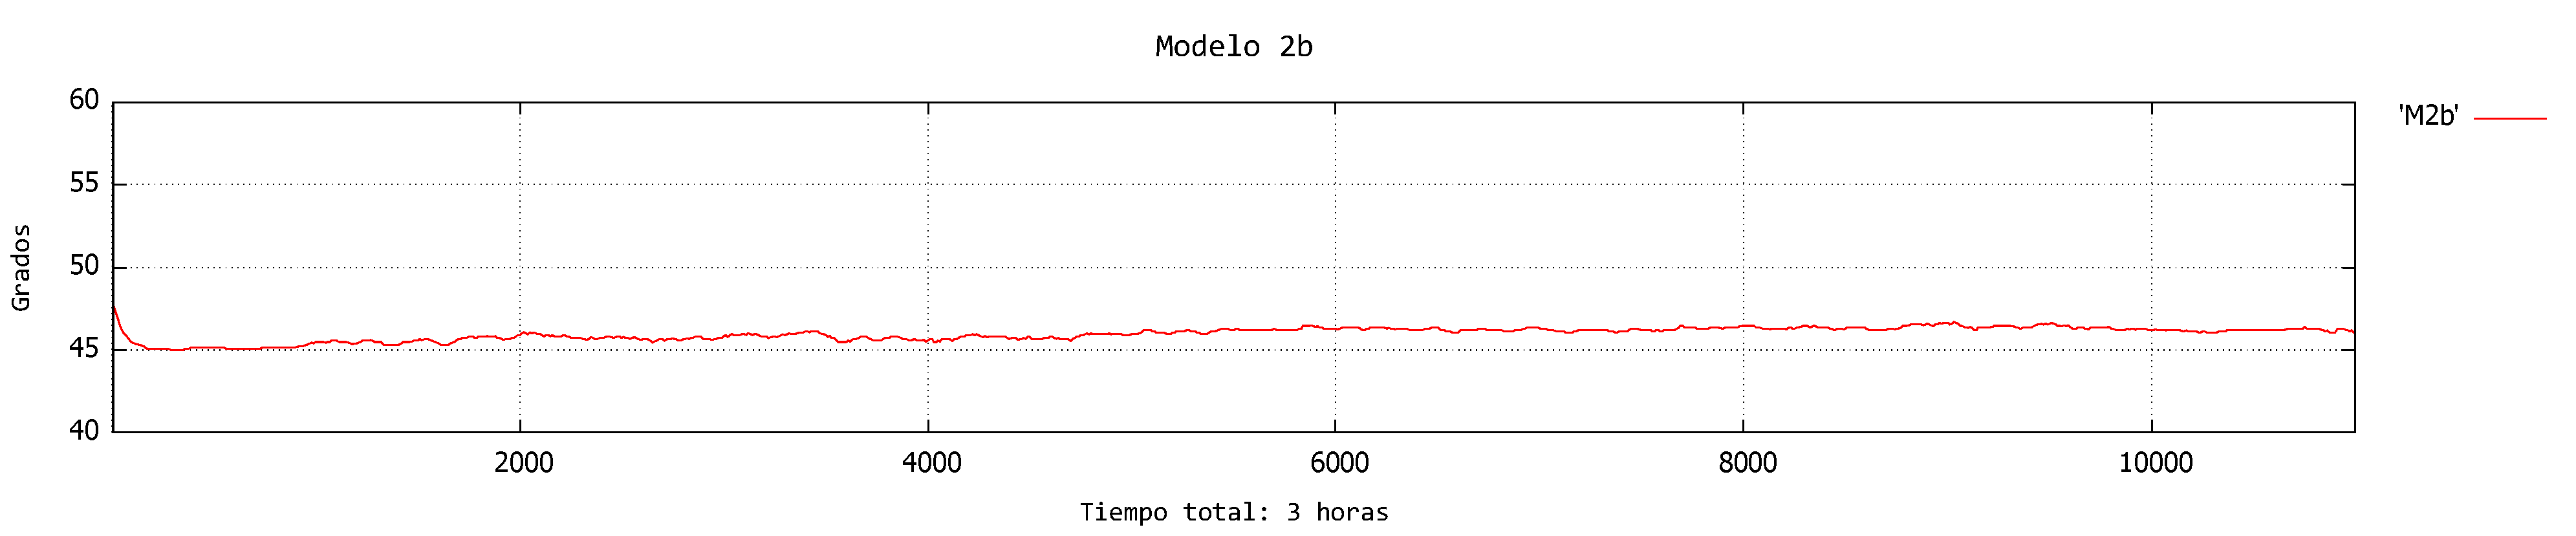
\includegraphics[width=160mm]{Test/Pr1_modelo2b.pdf}
   	\caption[Prueba 1, Modelo 2b]{Modelo 2b}
   \label{figure5.3}
\end{figure}

\begin{figure}[H]
	\centering
  	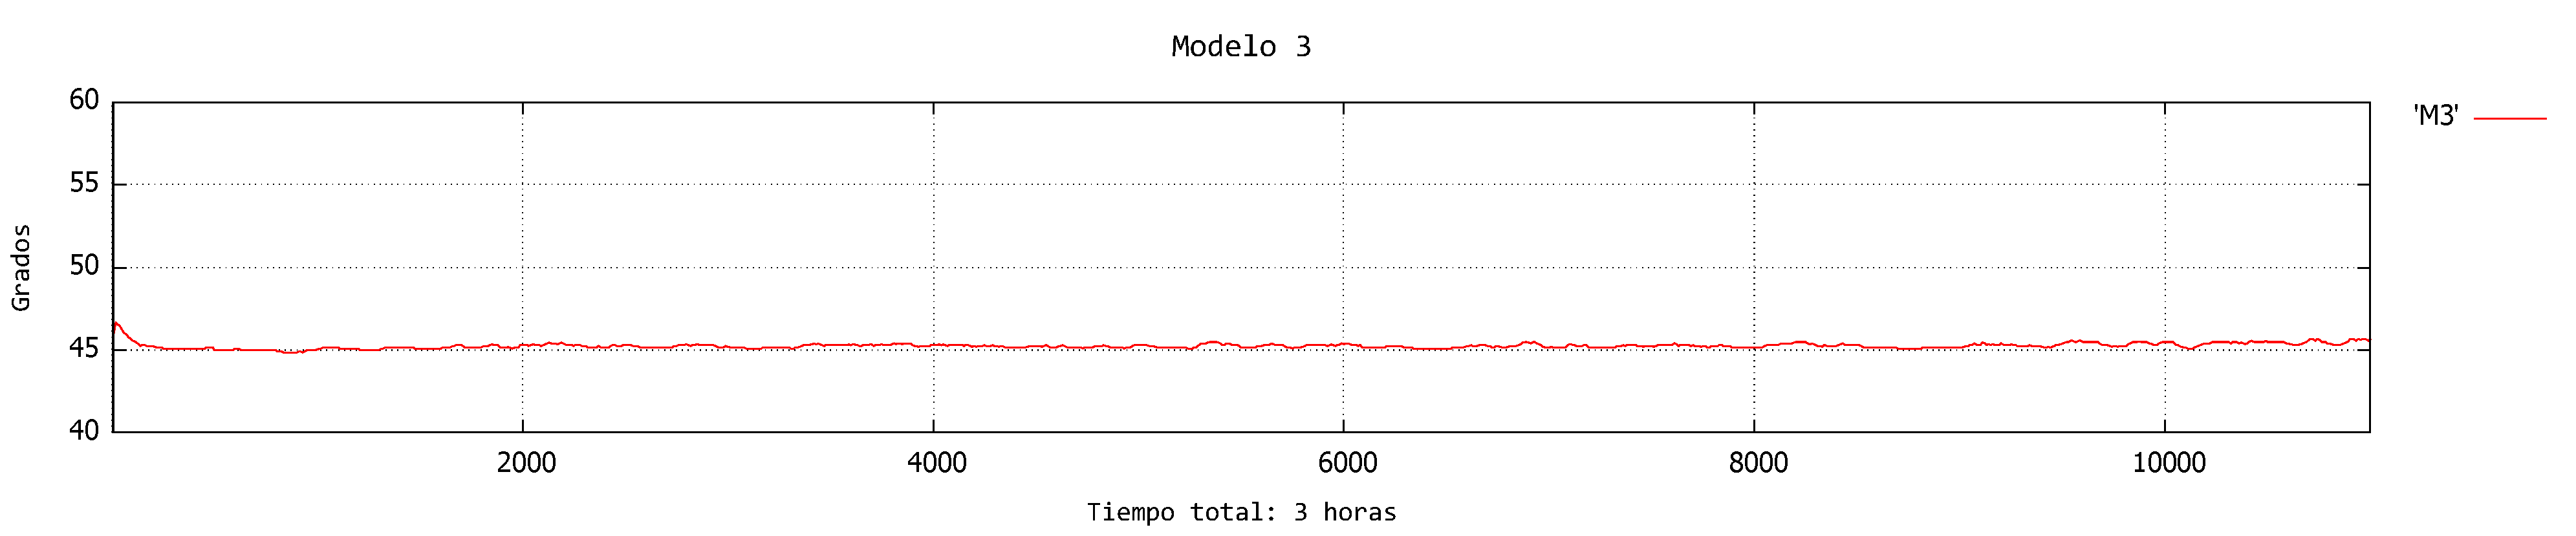
\includegraphics[width=160mm]{Test/Pr1_modelo3.pdf}
   	\caption[Prueba 1, Modelo 3]{Modelo 3}
   \label{figure5.4}
\end{figure}

\subsection{Conclusiones}
\paragraph{}

Se puede comprobar que tanto el modelo 2b como el modelo 3 son los que obtienen unos mejores resultados, en todo caso, en todos ellos, el sistema se mantiene estable durante toda la prueba, con muy poca variación entre sus temperaturas máxima y mínima. El modelo 2 registra unos valores cercanos a los sesenta grados, con lo que es sin duda el peor de los tres.

\section{Prueba 2}
\label{makereference5.4}
\subsection{Escenario}
\paragraph{}

En esta prueba hay tres Raspberrys trabajando de forma simultánea, cada una de ellas mantiene sus cuatro cores trabajando a máximo rendimiento, el tiempo total de las pruebas es nuevamente de tres horas, igual que en la prueba anterior el periodo de muestreo es de diez segundos y en cada gráfica muestra el tiempo total expresado en segundos. La temperatura ambiente, en este caso, oscila entre los quince y dieciocho grados. Una de las Raspberrys dispone de un disipador de calor, en las gráficas, esta se identifica con la letra D al lado de su nombre.

\subsection{Resultados}
\paragraph{}

\begin{figure}[H]
	\centering
  	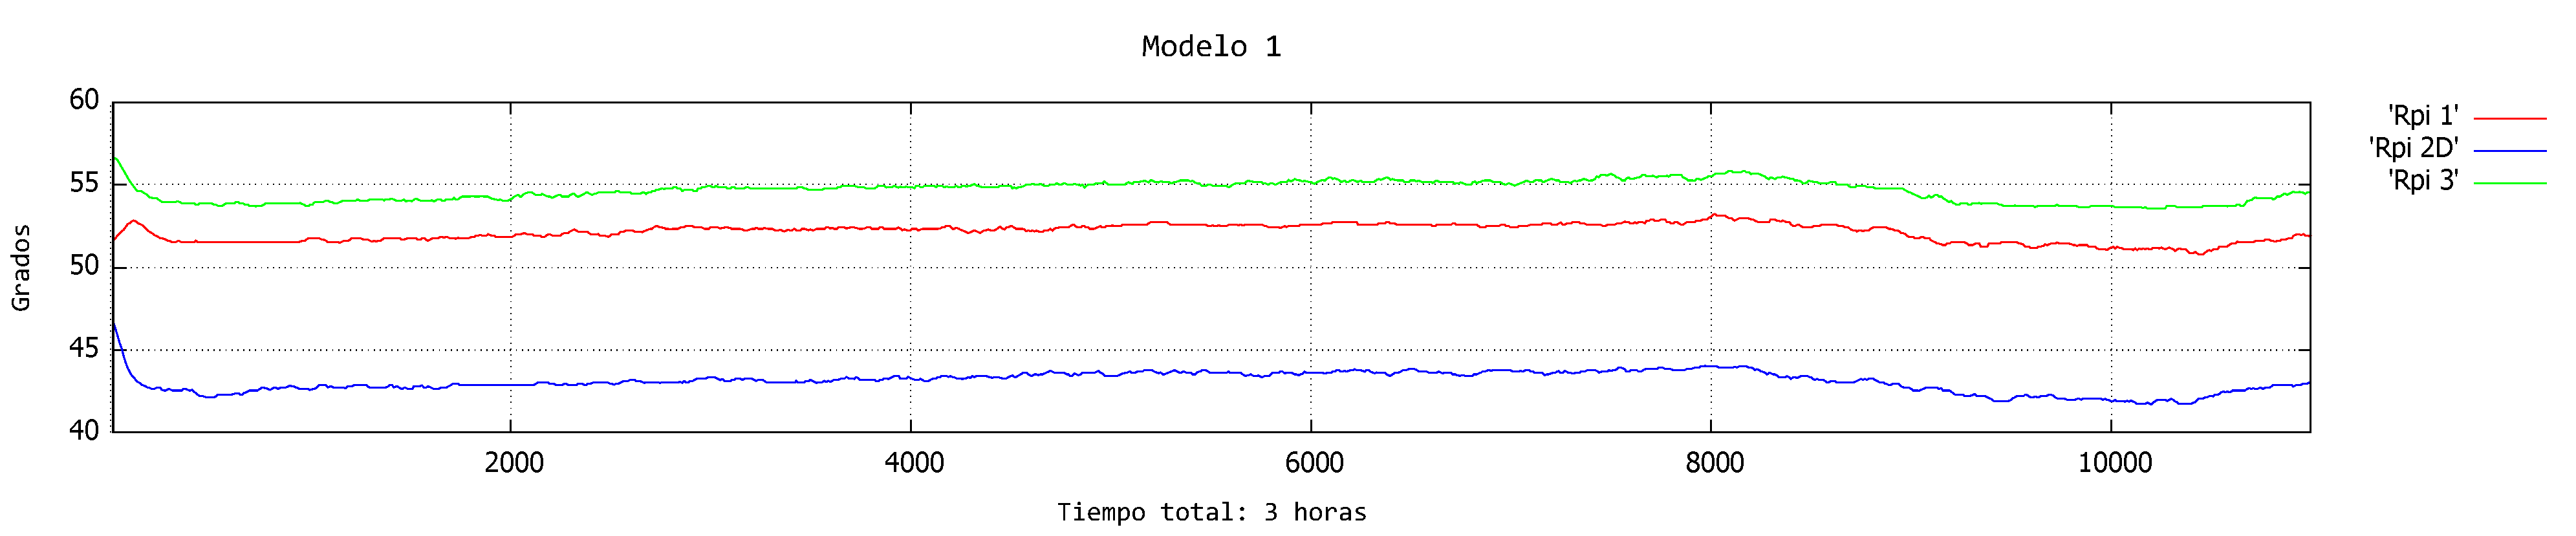
\includegraphics[width=160mm]{Test/pr2_modelo1.pdf}
   	\caption[Prueba 2, Modelo 1]{Modelo 1}
   \label{figure5.5}
\end{figure}

\begin{figure}[H]
	\centering
  	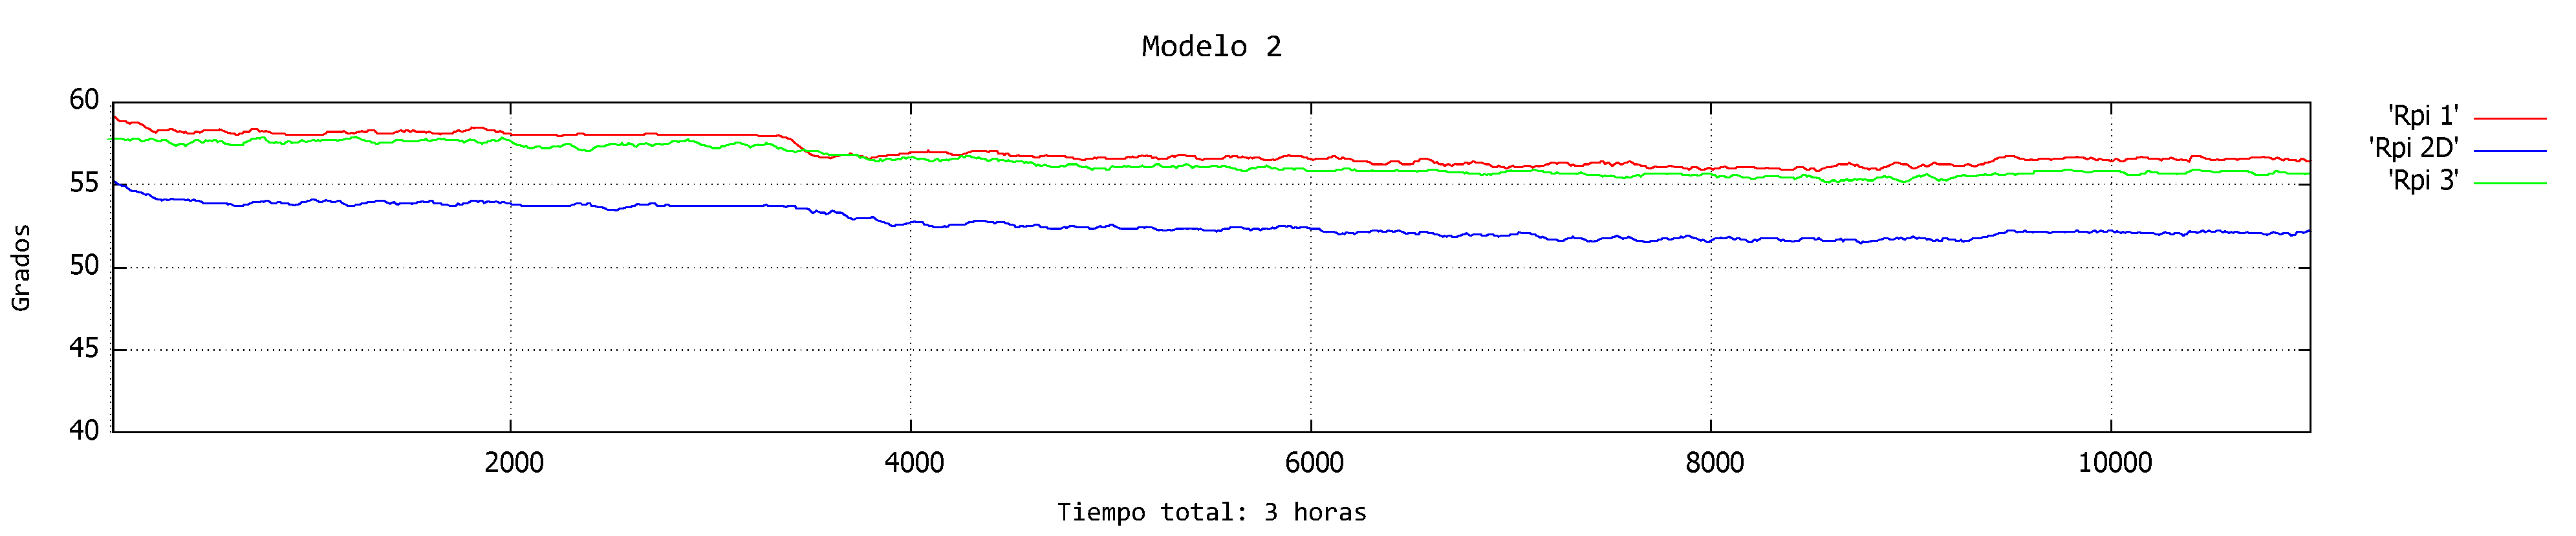
\includegraphics[width=160mm]{Test/pr2_modelo2.pdf}
   	\caption[Prueba 2, Modelo 2]{Modelo 2}
   \label{figure5.6}
\end{figure}

\begin{figure}[H]
	\centering
  	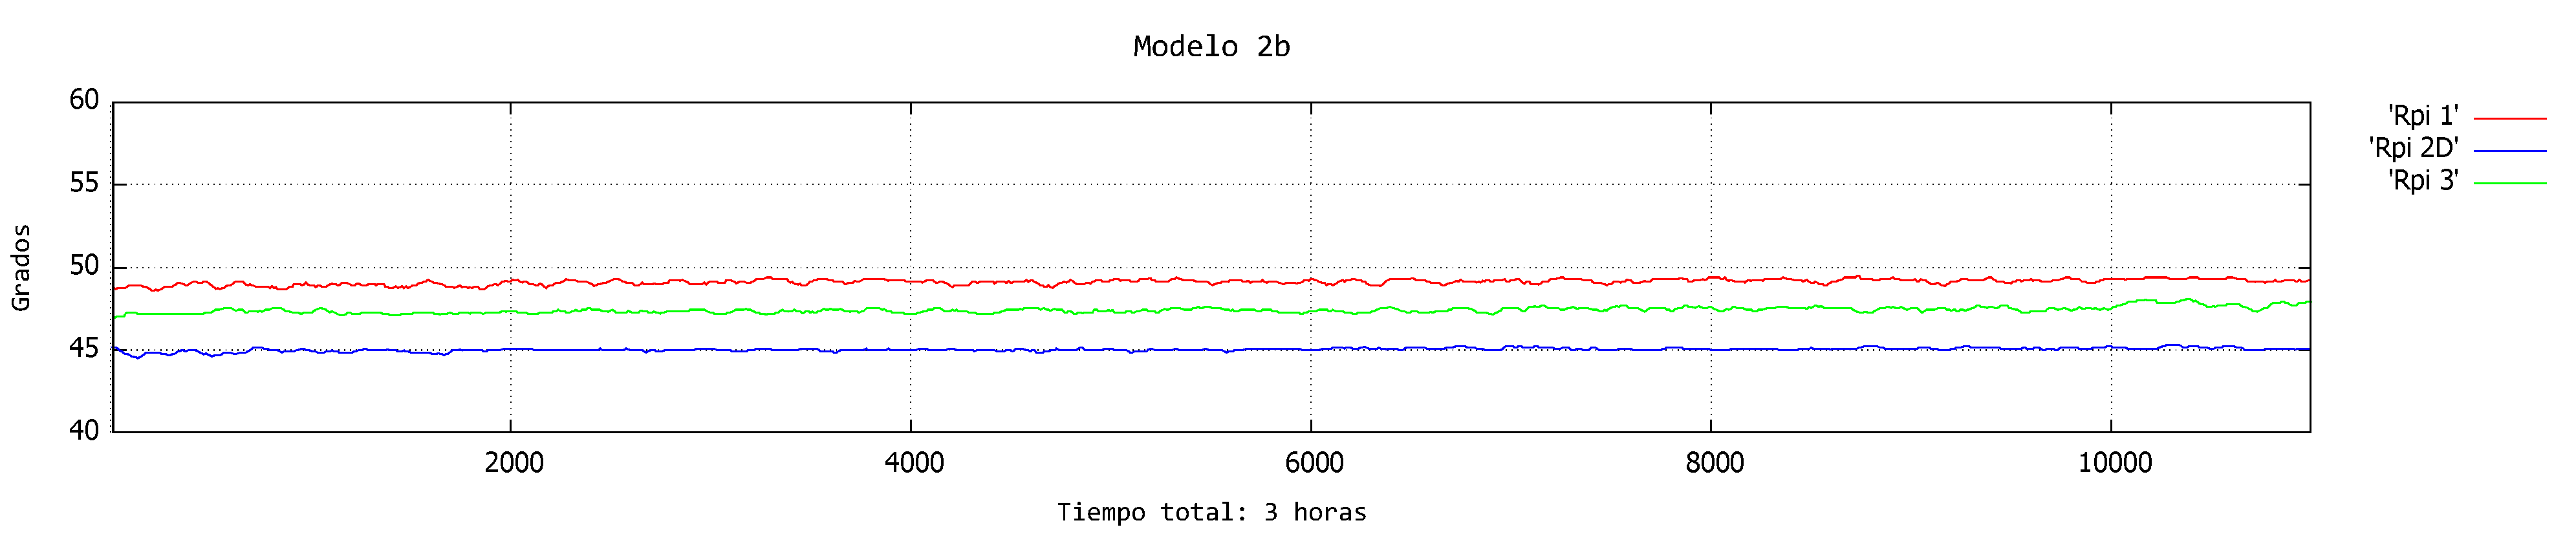
\includegraphics[width=160mm]{Test/pr2_modelo2b.pdf}
   	\caption[Prueba 2, Modelo 2b]{Modelo 2b}
   \label{figure5.7}
\end{figure}

\begin{figure}[H]
	\centering
  	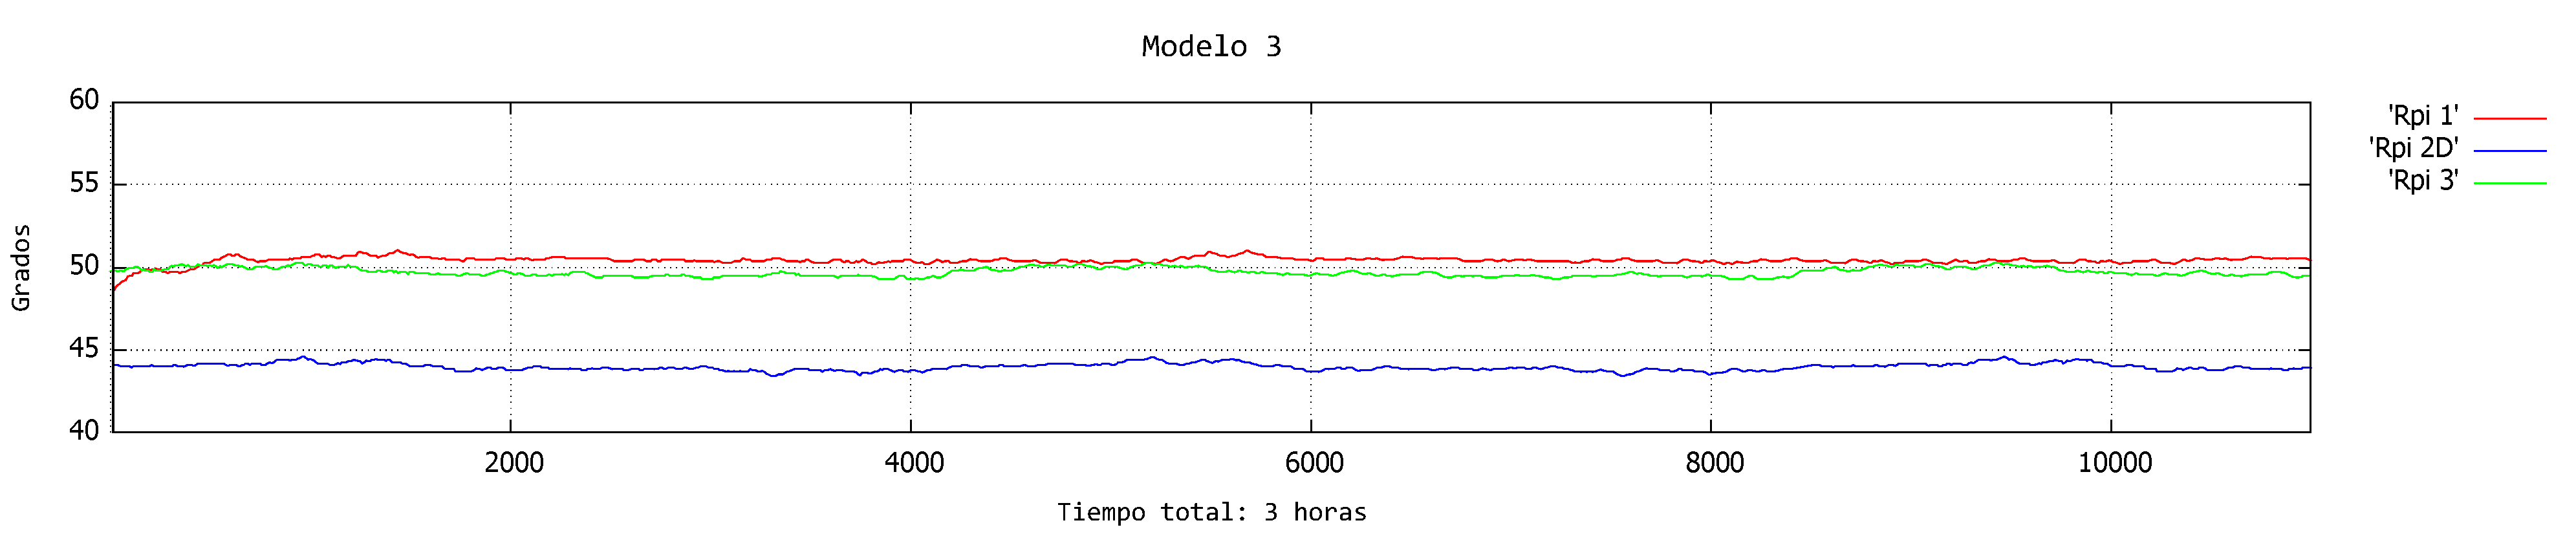
\includegraphics[width=160mm]{Test/pr2_modelo3.pdf}
   	\caption[Prueba 2, Modelo 3]{Modelo 3}
   \label{figure5.8}
\end{figure}

\subsection{Conclusiones}
\paragraph{}

Hemos comprobado que una buena corriente de aire hace que aquellos nodos que disponen de un disipador de calor instalado presenten unas temperaturas notablemente inferiores al resto. Sin embargo, como pasa en el modelo 2, figura \ref{figure5.6}, si la corriente no es eficiente, dicha mejora se ve severamente afectada.

De nuevo, los modelos 2b y 3, ofrecen unos resultados mejores, además se mantienen más estables durante toda la prueba. El modelo 1, figura \ref{figure5.5}, es en el que más variación de temperatura se observa entre Raspberrys con y sin disipadores. Nuevamente el modelo 2 tiene unas temperaturas superiores, cercanas a los sesenta grados.
Vemos además que el hecho de incluir más nodos de cómputo no afecta a las temperaturas medias de cada uno, ofreciendo resultados similares a los de la primera prueba.

\section{Prueba 3}
\label{makereference5.5}

\subsection{Escenario}
\paragraph{}

Finalmente en esta última prueba hay seis Raspberrys trabajando de forma simultánea, como en los casos anteriores, cada una de ellas mantiene sus cuatro cores trabajando en paralelo, el tiempo total de las pruebas es nuevamente de tres horas y el muestreo se realiza cada diez segundos. La temperatura ambiente oscila entre los dieciséis y diecisiete grados. Para esta prueba existen dos Raspberrys que disponen de disipadores de calor, identificadas nuevamente con la letra D en la gráfica.

\subsection{Resultados}
\paragraph{}

\begin{figure}[H]
	\centering
  	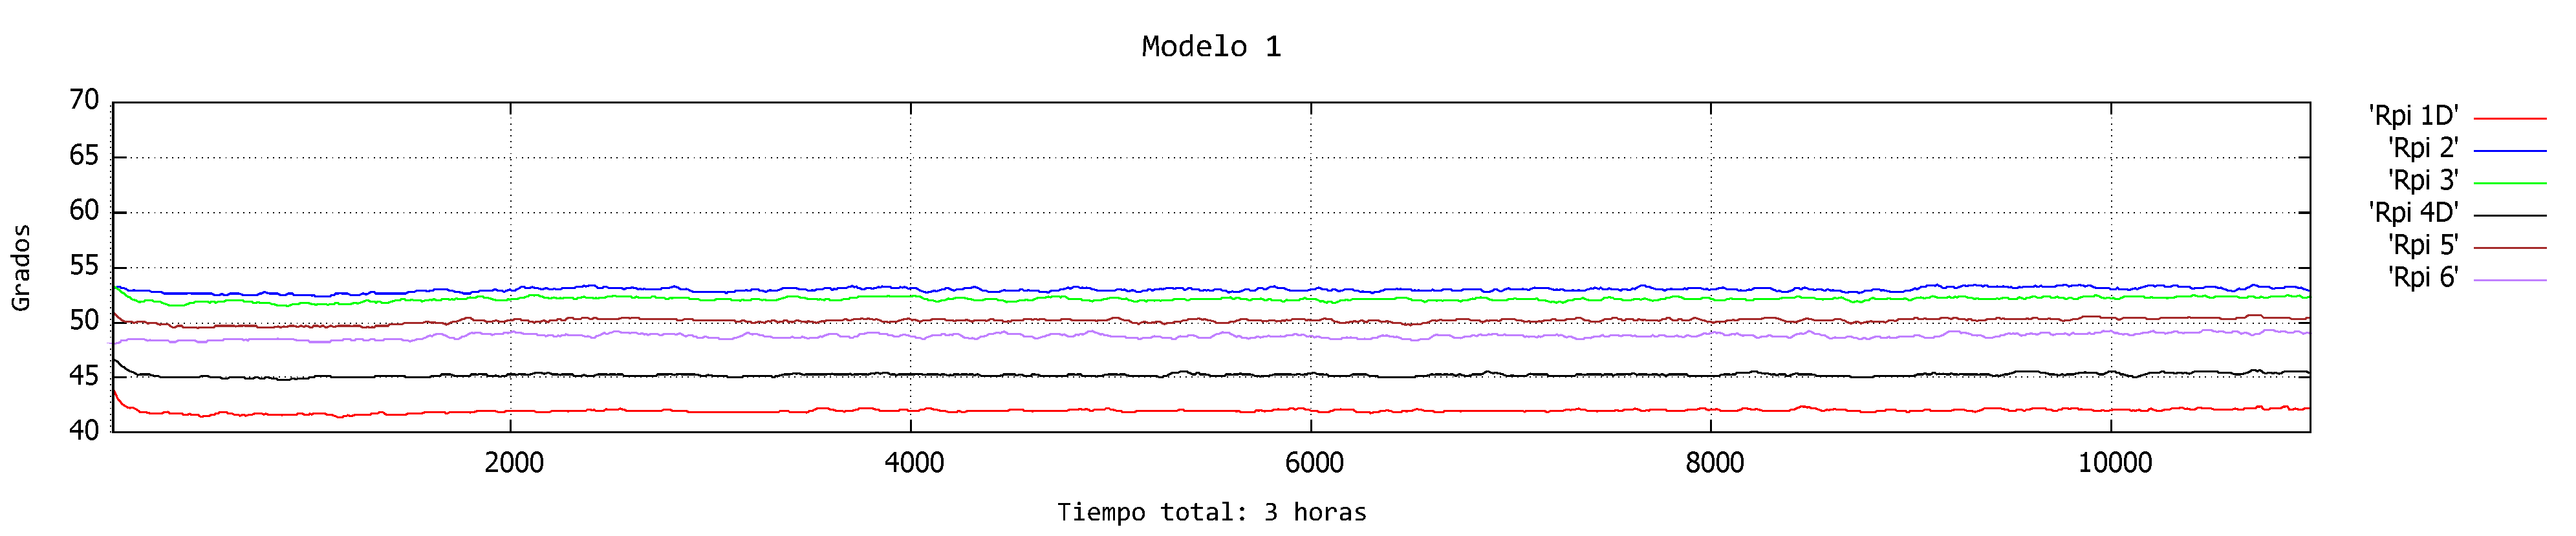
\includegraphics[width=160mm]{Test/pr3_modelo1.pdf}
   	\caption[Prueba 3, Modelo 1]{Modelo 1}
   \label{figure5.9}
\end{figure}


\begin{figure}[H]
	\centering
  	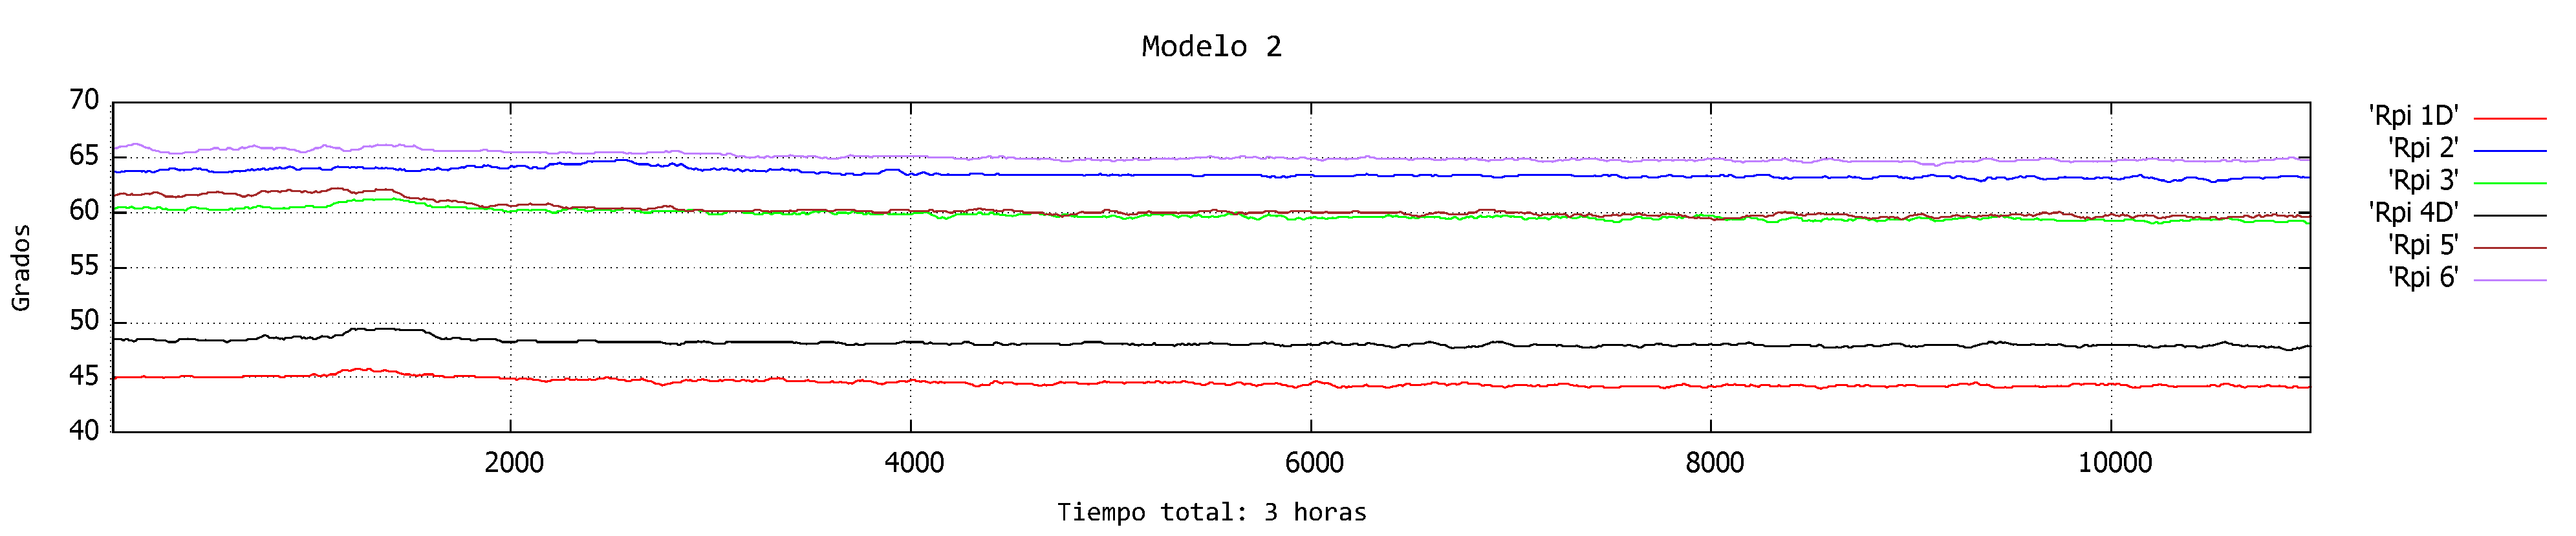
\includegraphics[width=160mm]{Test/pr3_modelo2.pdf}
   	\caption[Prueba 3, Modelo 2]{Modelo 2}
   \label{figure5.10}
\end{figure}

\begin{figure}[H]
	\centering
  	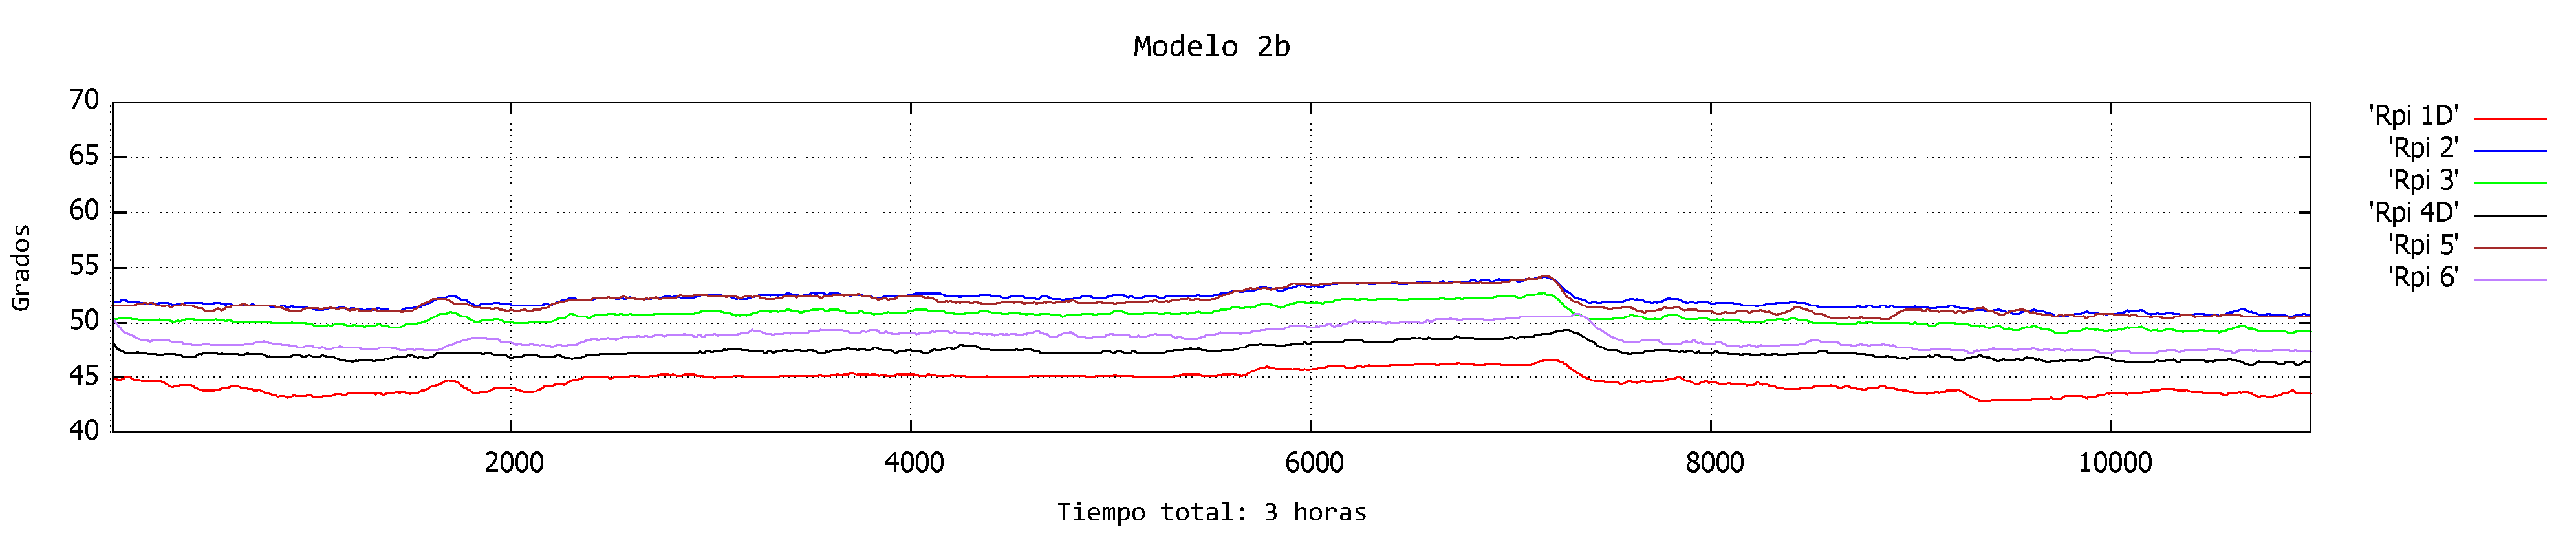
\includegraphics[width=160mm]{Test/pr3_modelo2b.pdf}
   	\caption[Prueba 3, Modelo 2b]{Modelo 2b}
   \label{figure5.11}
\end{figure}

\begin{figure}[H]
	\centering
  	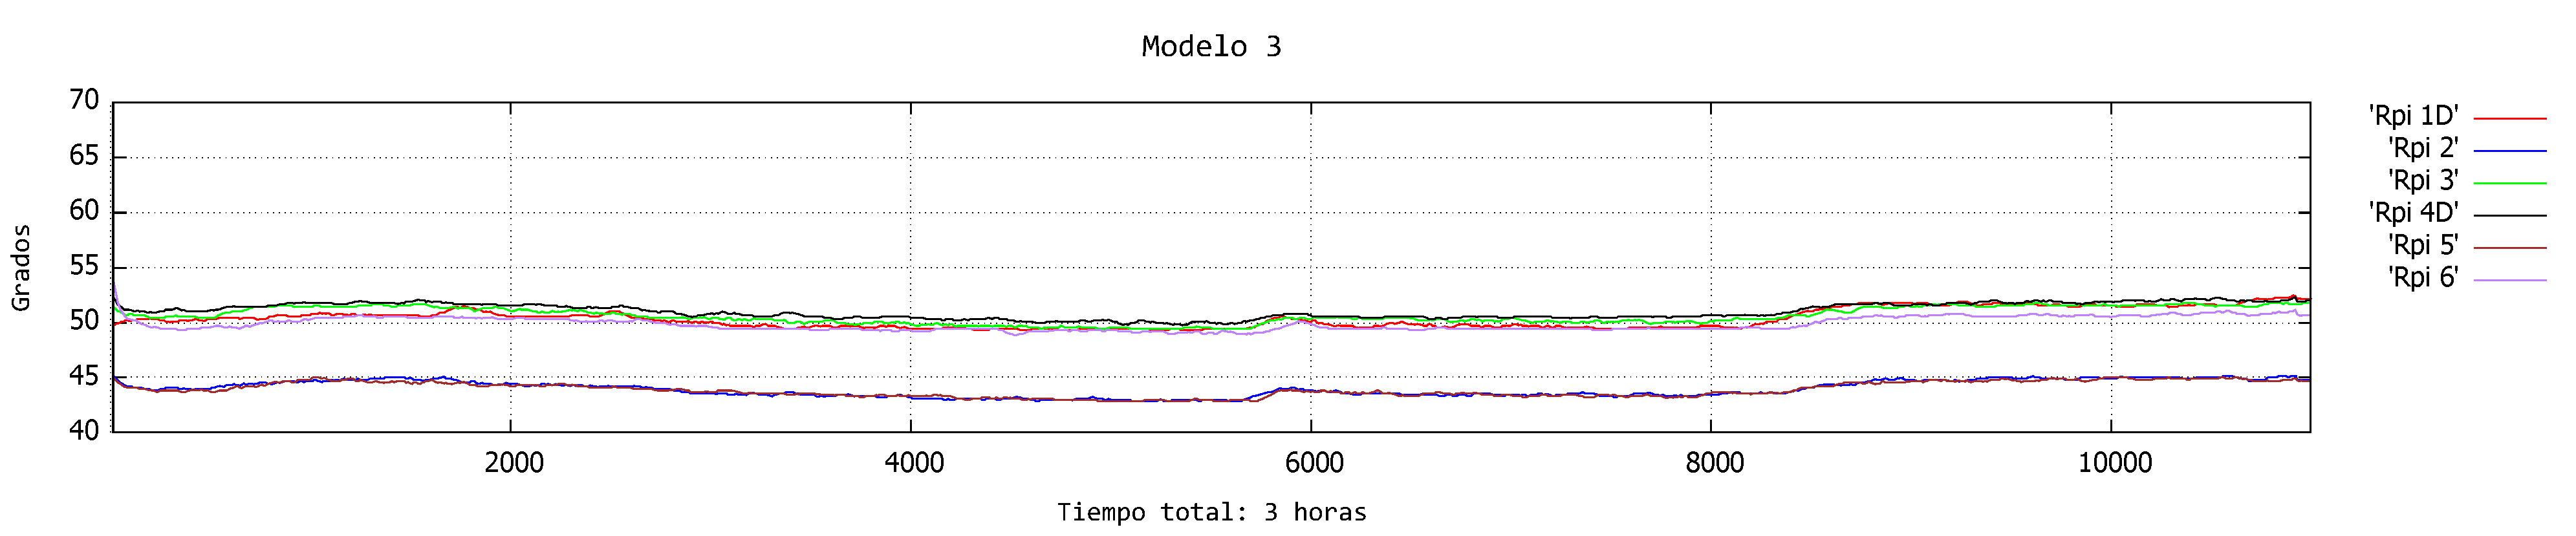
\includegraphics[width=160mm]{Test/pr3_modelo3.pdf}
   	\caption[Prueba 3, Modelo 3]{Modelo 3}
   \label{figure5.12}
\end{figure}

\subsection{Conclusiones}
\paragraph{}
En esta prueba hemos detectado que definitivamente el modelo 2 no cumple con las expectativas necesarias para el correcto funcionamiento del clúster, en él, las diferencias entre nodos con y sin disipador son muy notables y aquellas que no disponen de esta mejora arrojan unas temperaturas muy próximas a los ochenta grados, temperatura crítica de parada, por lo que podemos descartar este modelo para el desarrollo final.

Los otros tres modelos ofrecen unos resultados semejantes a las anteriores pruebas, particularmente el modelo 1 sigue mostrando gran diferencia entre los nodos con disipador. El modelo 2b, aunque ofrece algunas variaciones más notables durante la prueba, sigue manteniendo una relación parecida entre nodos, independientemente de que incluya o no disipadores.

El modelo 3 presenta los mejores resultados, manteniendo temperaturas bajas cercanas a los cincuenta grados y una notable diferencia entrelas Raspberrys que disponen de disipador, las cuales se mantienen en cuarenta y cinco grados. 

\section{Prueba 4}

\label{makereference5.6}
\subsection{Escenario}
\paragraph{}

El objetivo de esta última prueba es comprobar el comportamiento del sistema durante un periodo de tiempo largo. Se realizó sobre el modelo 1 durante venticuatro horas de forma ininterrumpida. El escenario es similar al de la prueba 3, con seis Raspberrys trabajando en paraleleo,  sin embargo, este muestreo se realiza cada sesenta segundos. No podemos certificar la temperatura ambiente para toda la prueba, pero calculamos que osciló entre los quince y dieciocho grados.

\subsection{Resultados}

\begin{figure}[H]
	\centering
  	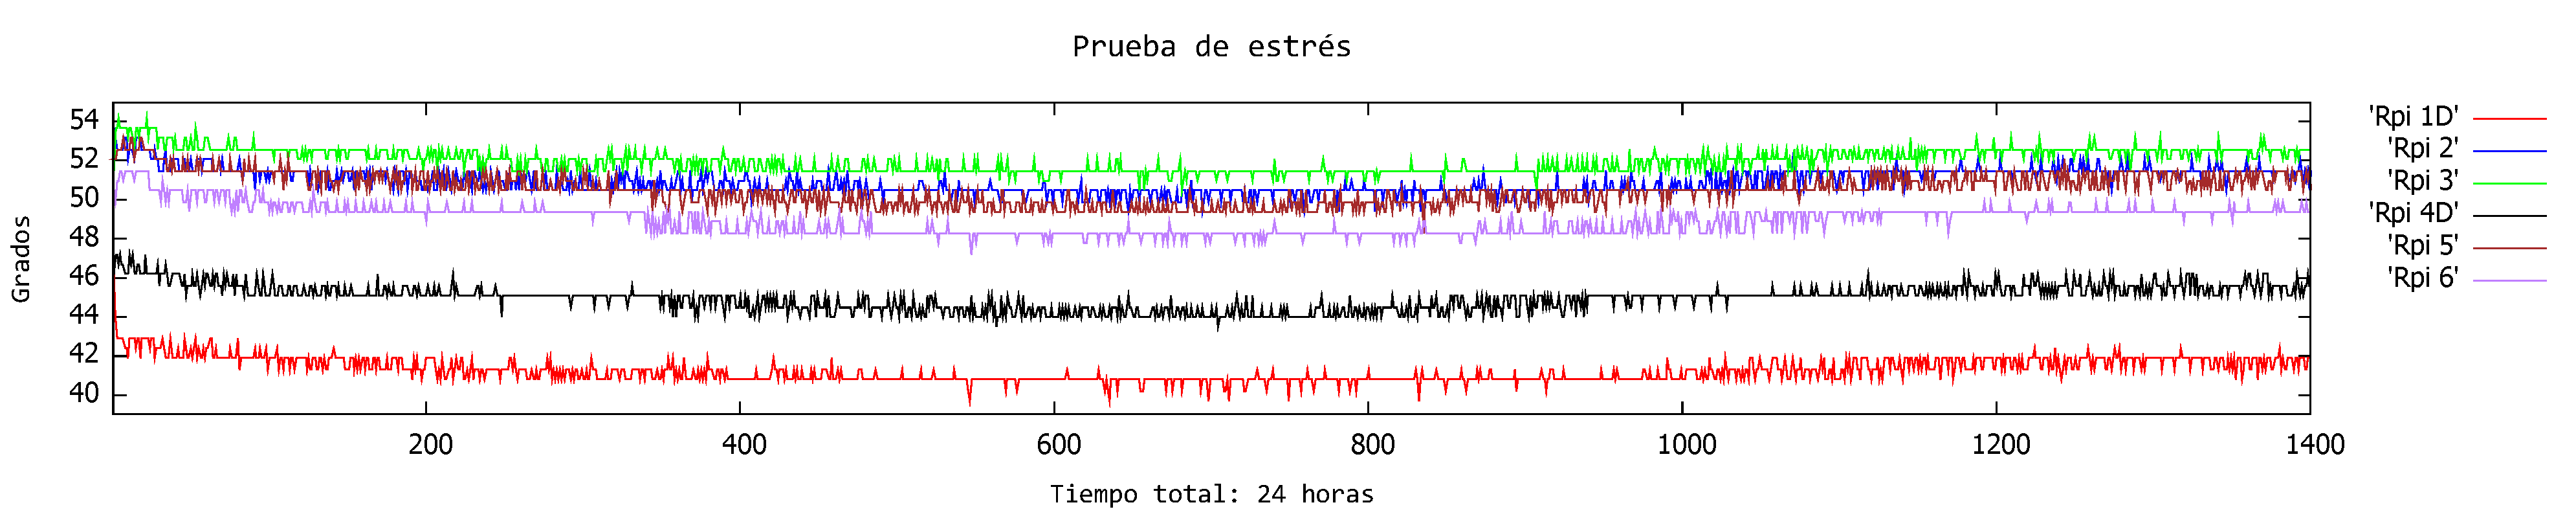
\includegraphics[width=175mm]{Test/pr4_estres.pdf}
   	\caption[Prueba 4, Prueba de estrés]{Resultados}
   \label{figure5.13}
\end{figure}

\subsection{Conclusiones}

Prueba de estrés

\section{Conclusiones generales}
\label{makereference5.7}
\paragraph{}

Durante el desarrollo de los test hemos podido apreciar algunos de los diferentes factores más influyentes sobre el sistema, a continuación, destacamos los que han sido más notorios:

\begin{enumerate}

\item Las \textit{corrientes de aire} tienen una gran afección, merece la pena dedicar parte del trabajo a buscar una eficiencia en la conducción de flujos de aire dentro del contenedor, una buena distribución de la entrada y salida de aire nos permite reducir el número de ventiladores y establecer un punto de partida para la disposición del resto de elementos.

\item Al contar con un gran número de cables, también es necesario combinar el punto anterior con la \textit{accesibilidad general a los dispositivos}, de esta manera, exponiendo las tarjetas SD conseguimos que no sea necesario abrir el contenedor para acceder a cada uno de los nodos.

\item La \textit{temperatura ambiente} es otro de los factores influyentes en el comportamiento general, aunque menos notorio, se pueden apreciar alteraciones en todos los dispositivos sujetos a este efecto. Sería preciso que ésta se mantuviera lo más estable posible.

\item En cuanto a la \textit{robustez}, los resultados ofrecidos por la prueba de estrés, figura \ref{figure5.13}, muestran que el comportamiento ha sido similar al del resto de pruebas, independientemente del número de horas, por lo que podemos concluir que el sistema es fiable y poco propenso a las caídas repentinas por periodos largos de trabajo.

\item En las diferentes pruebas realizadas hemos observado que \textit{no existe una correlación entre tasa de trabajo completado y temperatura}. Aún así, con el fin de prolongar la vida útil de cada nodo, siempre es mejor mantener un rango de temperaturas bajo.

\item El uso de \textit{disipadores} es muy conveniente, son elementos de precio reducido, y con una distribución de aire adecuada aumentan tanto la vida útil del clúster, como el comportamiento de los nodos ante los cambios bruscos de temperatura ambiente. En el peor de los casos, todos los nodos que disponían de esta mejora ofrecieron unos resultados inferiores a los del resto.

\end{enumerate}
